\documentclass[tikz,border=6pt]{standalone}

% общий стиль (подключается через TEXINPUTS)
% tikz-style.tex (общий стиль для всех TikZ-картинок)
\RequirePackage[T1,T2A]{fontenc}
\RequirePackage[utf8]{inputenc}

% Palatino-подобный шрифт (как в MathJax часто воспринимается «более вытянутым»)
\RequirePackage{txfonts}
% txfonts даёт предупреждение по кириллице (T2A/txr не определён).
% Оставляем txfonts для математики, а текстовый шрифт возвращаем на Computer Modern,
% чтобы не искать T2A/txr и убрать предупреждения.
\renewcommand{\rmdefault}{cmr}
\renewcommand{\sfdefault}{cmss}
\renewcommand{\ttdefault}{cmtt}

\RequirePackage{tikz}
\RequirePackage{xcolor}
\usetikzlibrary{calc}

% цвета
\definecolor{lightgreen}{RGB}{214,234,214}
\definecolor{darkgreen}{HTML}{0B7A0B}
\definecolor{darkred}{HTML}{DF0000}

\definecolor{midgreen}{HTML}{2E9B2E}
\definecolor{palegreen}{RGB}{235,246,235}
\definecolor{olivegreen}{HTML}{3E6B2F}

\definecolor{lightred}{RGB}{255,220,220}
\definecolor{midred}{HTML}{E04545}
\definecolor{darkred2}{HTML}{A80000}

\definecolor{lightblue}{RGB}{220,232,255}
\definecolor{midblue}{HTML}{2E5BD6}
\definecolor{darkblue}{HTML}{0B2E8A}

\definecolor{lightgray}{RGB}{240,240,240}
\definecolor{midgray}{RGB}{170,170,170}
\definecolor{darkgray}{RGB}{80,80,80}

\definecolor{vtxfill}{RGB}{86,193,255}
\definecolor{vennfill}{RGB}{220,232,255}


% единый набор стилей TikZ
\tikzset{
    lab/.style={
        font=\fontsize{24}{32}\selectfont
    }
}


\begin{document}
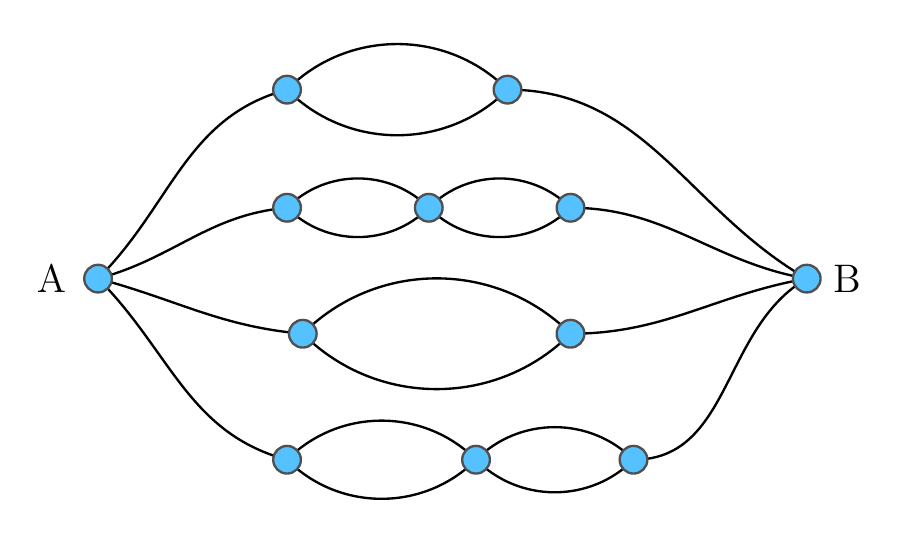
\begin{tikzpicture}[x=1cm,y=1cm, line cap=round, line join=round]

\tikzset{
  main/.style={draw=black, line width=0.85pt},
  vtx/.style={circle, draw=darkgray, fill=vtxfill, line width=0.85pt, minimum size=10pt, inner sep=0pt},
  vlab/.style={font=\Large},
}

\coordinate (A) at (0,0);
\coordinate (U1) at (2.4,2.4);
\coordinate (U2) at (5.2,2.4);
\coordinate (S1) at (2.4,0.9);
\coordinate (S2) at (4.2,0.9);
\coordinate (S3) at (6.0,0.9);
\coordinate (T1) at (2.6,-0.7);
\coordinate (T2) at (6.0,-0.7);
\coordinate (L1) at (2.4,-2.3);
\coordinate (L2) at (4.8,-2.3);
\coordinate (L3) at (6.8,-2.3);
\coordinate (B) at (9.0,0);

% edges A -> four corridors
\draw[main] (A) to[out=45,in=195] (U1);
\draw[main] (A) to[out=15,in=185] (S1);
\draw[main] (A) to[out=-15,in=175] (T1);
\draw[main] (A) to[out=-45,in=165] (L1);

% верхний коридор (2 параллельные дуги)
\draw[main] (U1) to[out=45,in=135] (U2);
\draw[main] (U1) to[out=-45,in=-135] (U2);

% второй коридор (2 x 2)
\draw[main] (S1) to[out=45,in=135] (S2);
\draw[main] (S1) to[out=-45,in=-135] (S2);

\draw[main] (S2) to[out=45,in=135] (S3);
\draw[main] (S2) to[out=-45,in=-135] (S3);

% третий коридор (2 параллельные дуги)
\draw[main] (T1) to[out=45,in=135] (T2);
\draw[main] (T1) to[out=-45,in=-135] (T2);

% нижний коридор (2 x 2)
\draw[main] (L1) to[out=45,in=135] (L2);
\draw[main] (L1) to[out=-45,in=-135] (L2);

\draw[main] (L2) to[out=45,in=135] (L3);
\draw[main] (L2) to[out=-45,in=-135] (L3);

% to B
\draw[main] (U2) to[out=0,in=150] (B);
\draw[main] (S3) to[out=0,in=170] (B);
\draw[main] (T2) to[out=0,in=-170] (B);
\draw[main] (L3) to[out=0,in=-150] (B);

% vertices
\node[vtx] at (A) {};
\node[vtx] at (U1) {};
\node[vtx] at (U2) {};
\node[vtx] at (S1) {};
\node[vtx] at (S2) {};
\node[vtx] at (S3) {};
\node[vtx] at (T1) {};
\node[vtx] at (T2) {};
\node[vtx] at (L1) {};
\node[vtx] at (L2) {};
\node[vtx] at (L3) {};
\node[vtx] at (B) {};

% labels
\node[vlab, left=8pt] at (A) {A};
\node[vlab, right=6pt] at (B) {B};

\end{tikzpicture}
\end{document}
